%!TEX root=../document.tex

\section{Ergebnisse}
\label{sec:Ergebnisse}
\subsection{Über OpenStack}
Der erste Schritt für mich war es, herauszufinden was OpenStack eigentlich bzw. was es macht.

OpenStack ist eine Software, welche normalerweise auf einem Server in einem Netzwerk läuft, um virtuelle Instanzen bereitzustellen. Auf diesem Server liegen beliebig viele Images, mit welchen virtuelle Maschinen erstellt werden können, um Rechenleistung auszulagern, Stichwort \glqq Cloud-Computing\grqq
\subsection{Installation}
Zuerst wurde versucht Openstack als Docker-Container zu starten. Dies war allerdings unerfolgreich, da Docker keine komplette Systemumgebung virtualisiert, sondern direkt auf den RAM, Speicher, Prozessor, Bus, etc. zugreift. Dies hat dazu geführt, dass eine virtuelle Maschine erstellt werden musste auf welcher CentOS läuft. Es wurde spezifisch ein CentOS Image gewählt, welches lediglich auf der Kommandozeile agiert, um kostbare Rechenleistung zu sparen. 

Ein Problem welches sehr oft aufgetreten ist, ist dass die virtuelle Maschine keine IP zugewiesen bekommen hat vom DHCP Server. Gelöst wurde das Problem indem eine neue IP angefragt wurde:

\begin{lstlisting}[language=bash]
sudo dhclient -r
sudo dhclient
\end{lstlisting}

Weiters war das Keyboardlayout falsch gesetzt, was mit folgendem Befehl korrigiert wurde:

\begin{lstlisting}[language=bash]
sudo loadkeys de
\end{lstlisting}

Um besser mit der virtualisierten Maschine zu interagieren, wurde sich per ssh auf die Maschine verbunden:

\begin{minipage}{\linewidth}
	\centering
	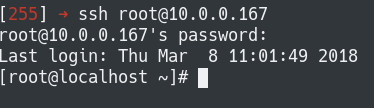
\includegraphics[width=0.8\linewidth]{images/ssh}
	\figcaption{Per ssh auf die CentOS virtuelle Maschine zugreifen}
\end{minipage}

Nach der Installation des Betriebssystems, wurde sich nach dem gegeben Tutorial \cite{Packstac62:online} orientiert. 

Der erste Schritt war es die Firewall auszuschalten, den NetworkManager zu stoppen und das Netzwerk neu zu starten, um Komplikationen zu vermeiden:

\begin{lstlisting}[language=bash]
sudo systemctl disable firewalld
sudo systemctl stop firewalld
sudo systemctl disable NetworkManager
sudo systemctl stop NetworkManager
sudo systemctl enable network
sudo systemctl start network
\end{lstlisting}

Im nächsten Schritt wurden alle nötigen Repositories installiert und runtergeladen, und schließlich ein Systemupdate durchgeführt:

\begin{lstlisting}[language=bash]
sudo yum install -y https://rdoproject.org/repos/rdo-release.rpm
sudo yum install -y centos-release-openstack-queens
yum-config-manager --enable openstack-queens
sudo yum update -y
\end{lstlisting}

Weiters wurde das Package openstack-packstack installiert, mit welchem OpenStack aufgesetzt wird:

\begin{lstlisting}[language=bash]
sudo yum install -y openstack-packstack
\end{lstlisting}

Der letzte Schritt ist alles starten zu lassen durch den Befehl:

\begin{lstlisting}[language=bash]
sudo packstack --allinone
\end{lstlisting}

Anschließend kann folgende Ausgabe erwartet werden:

\begin{minipage}{\linewidth}
	\centering
	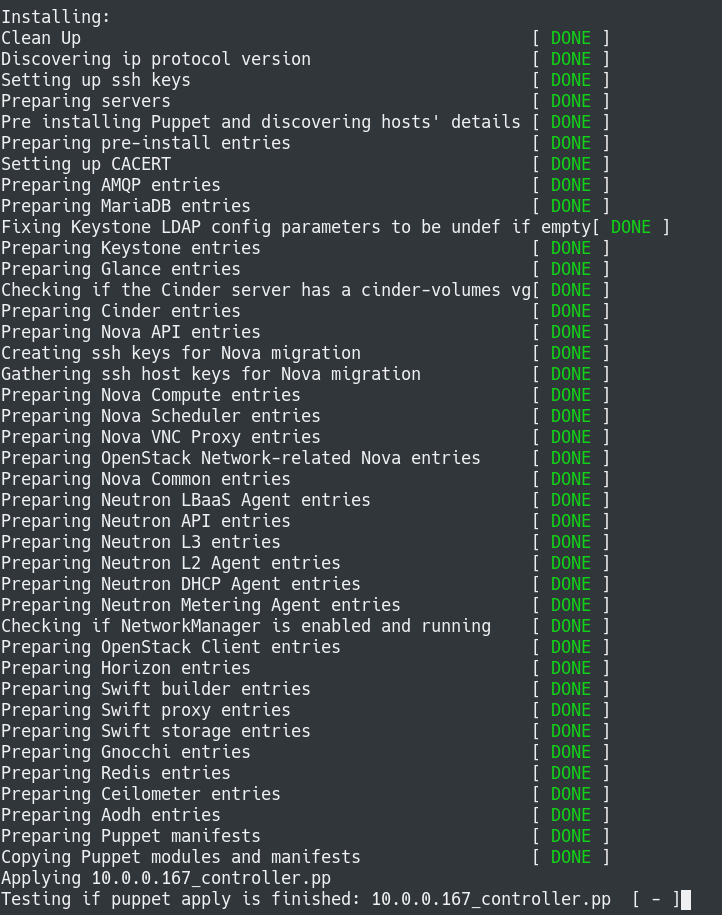
\includegraphics[width=0.53\linewidth]{images/packstack}
	\figcaption{Packstack wurde ausgeführt}
\end{minipage}

Nach sehr langer Wartezeit sieht man nun folgende Ausgabe um sich schließlich anzumelden:

\begin{minipage}{\linewidth}
	\centering
	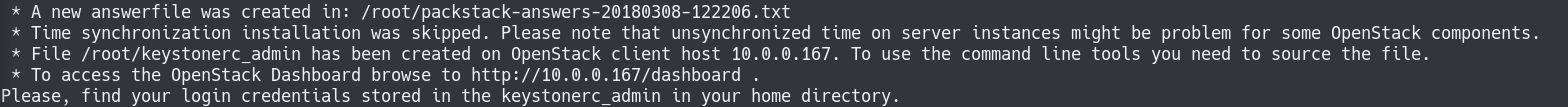
\includegraphics[width=1\linewidth]{images/packstackdone}
	\figcaption{Anweisungen für OpenStack werden ausgegeben}
\end{minipage}

\subsection{Login}
Anschließend sind die Anmeldedaten im File \verb|keystonerc_admin| zu finden:

\begin{minipage}{\linewidth}
	\centering
	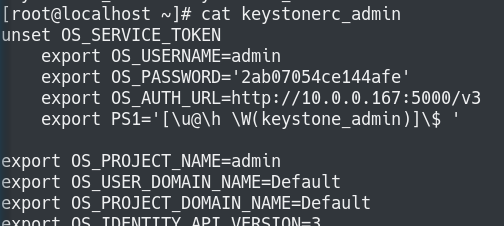
\includegraphics[width=.8\linewidth]{images/keystore}
	\figcaption{Passwort für Admin}
\end{minipage}

Wenn man nun im Browser \verb|http://10.0.0.167/dashboard/| besucht, kann man sich als admin einloggen:

\begin{minipage}{\linewidth}
	\centering
	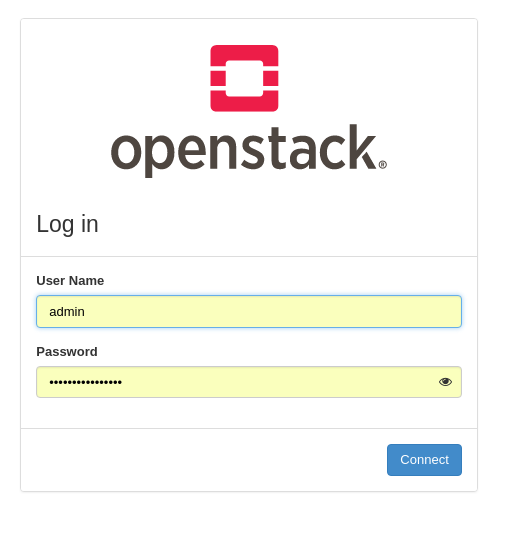
\includegraphics[width=.5\linewidth]{images/login}
	\figcaption{Login als Admin mit ausgelesenem Passwort}
\end{minipage}

\subsection{Image erstellen}
Nach dem Login, ist der erste Schritt ein Image zu erstellen. Dafür wurde ein CentOS image genommen, welches im Format \verb|QCOW2| bereitgestellt werden muss. 

Unter Project/Compute/Images kann auf \textbf{Create Image} gedrückt werden. Dort wird als nächstes der Image Name, die Image Datei und das Format angegeben:

\begin{minipage}{\linewidth}
	\centering
	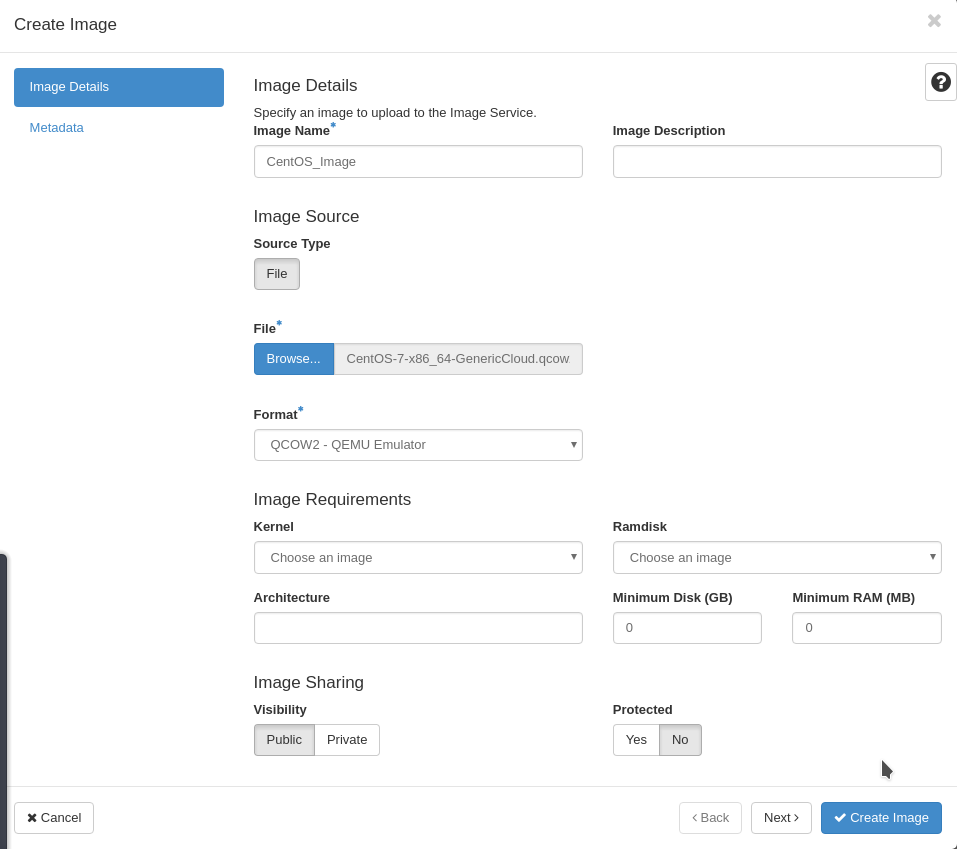
\includegraphics[width=.8\linewidth]{images/createimage}
	\figcaption{Image erstellen}
\end{minipage}
\subsection{Netzwerk erstellen}
Unter Project/Network/Networks kann ein neues Netzwerk durch den Button \textbf{Create Network} hinzugefügt werden. Hier wird als erstes der Name angegeben:

\begin{minipage}{\linewidth}
	\centering
	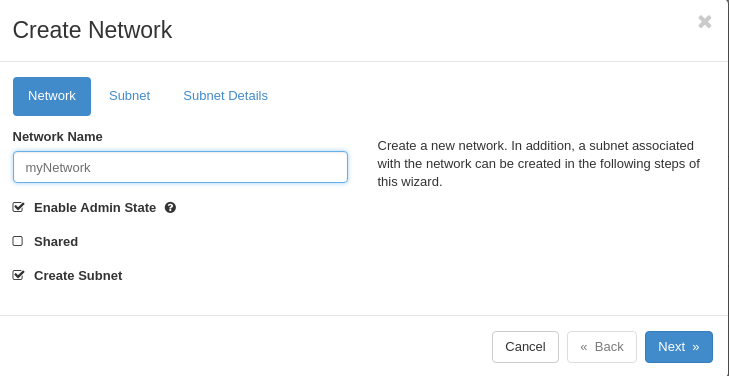
\includegraphics[width=.8\linewidth]{images/networkname}
	\figcaption{Netzwerkname angeben}
\end{minipage}

Als nächstes muss ein Subnet angegeben, sowie die Netzwerkadresse und die Gateway Adresse. In meinem Fall hab ich als Adresse \verb|192.168.0.0/24| und als Gateway standardmäßig \verb|192.168.0.1| gewählt:

\begin{minipage}{\linewidth}
	\centering
	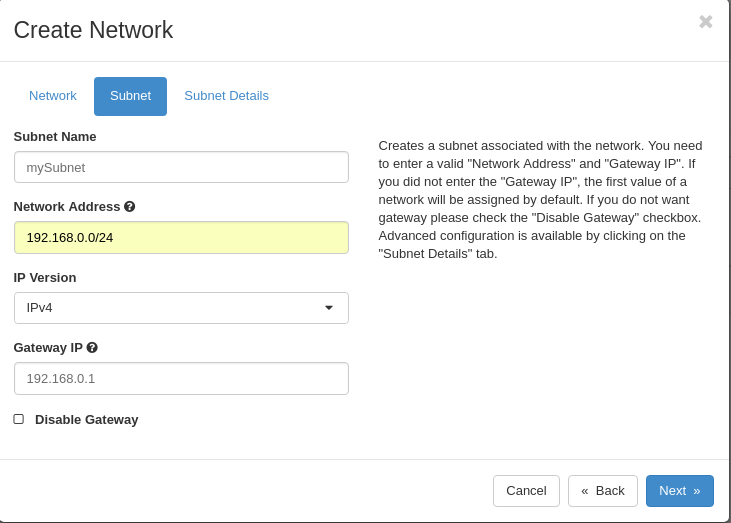
\includegraphics[width=.8\linewidth]{images/networksubnet}
	\figcaption{Subnet erstellen}
\end{minipage}

Weiters können noch andere Optionen angegeben werden:

\begin{minipage}{\linewidth}
	\centering
	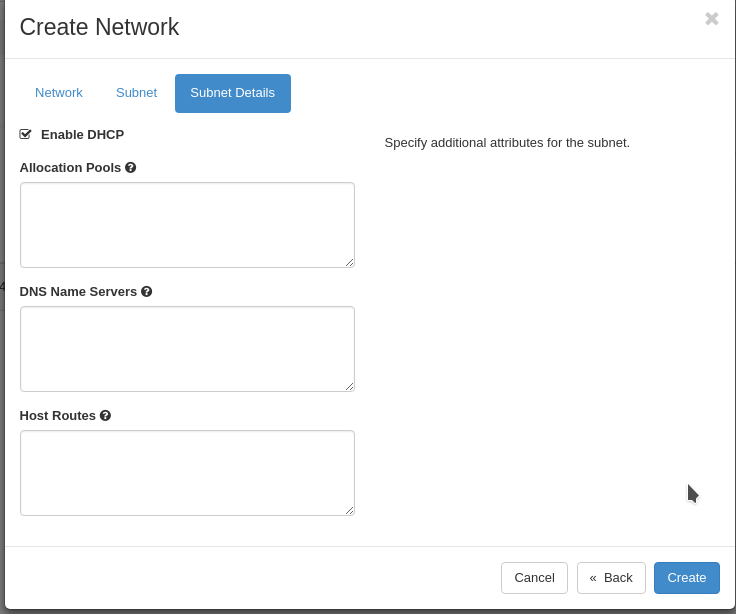
\includegraphics[width=.8\linewidth]{images/networkextra}
	\figcaption{Weitere Netzwerkinformationen angeben}
\end{minipage}

Danach kann unter Project/Network/Network Topology die Netzwerktopologie eingesehen werden:

\begin{minipage}{\linewidth}
	\centering
	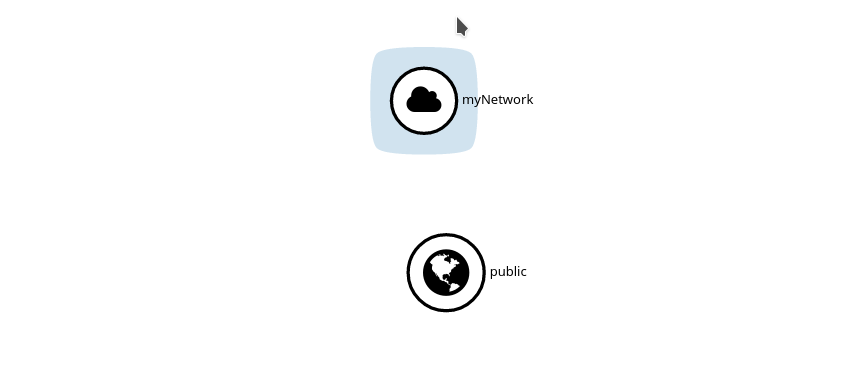
\includegraphics[width=.8\linewidth]{images/topologie}
	\figcaption{Netzwerktopologie}
\end{minipage}

\subsection{Instanz erstellen}
Nachdem ein Netzwerk und ein Image erstellt wurde, kann eine Instanz unter Project/Compute/Instances eine CentOS Instanz erstellt werden in dem definierten Netzwerk.

Dafür wird erstmals auf den Button \textbf{Launch Instance} gedrückt. Der erste Schritt ist einen Namen anzugeben:

\begin{minipage}{\linewidth}
	\centering
	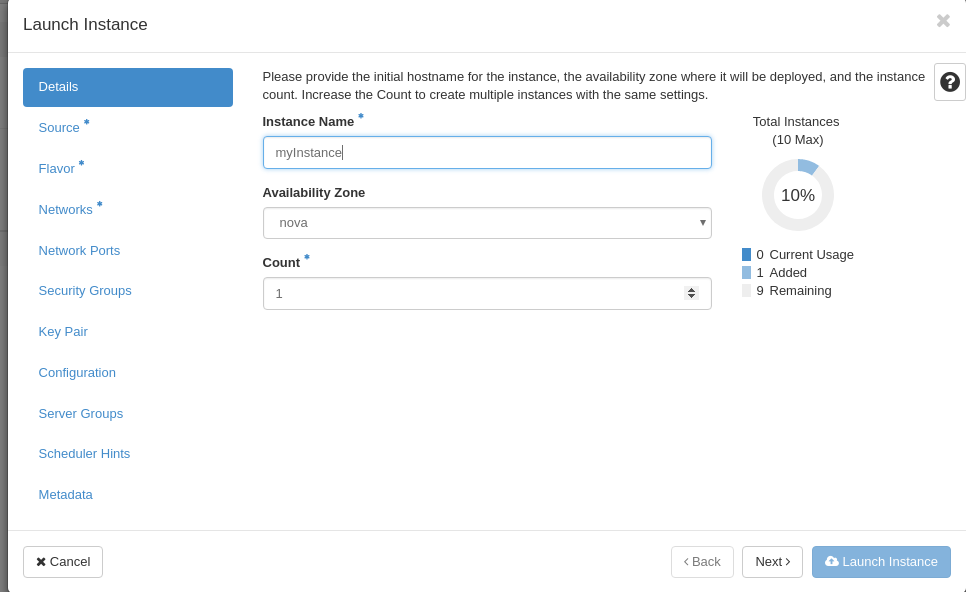
\includegraphics[width=.8\linewidth]{images/instancename}
	\figcaption{Instanznamen angeben}
\end{minipage}

Danach muss das vorhin definierte Image ausgewählt werden:

\begin{minipage}{\linewidth}
	\centering
	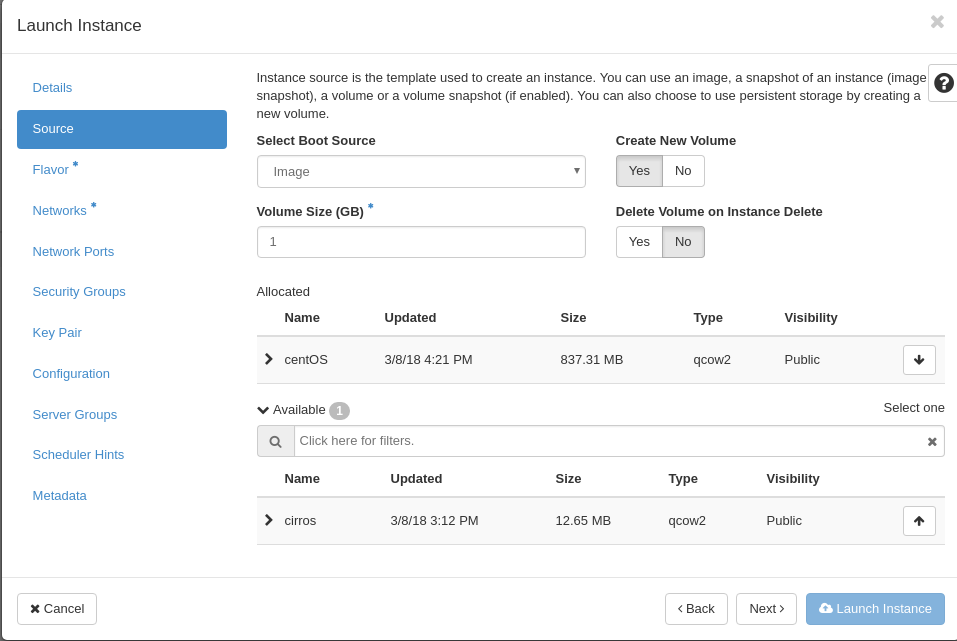
\includegraphics[width=.7\linewidth]{images/instanceimage}
	\figcaption{Image für Instanz auswählen}
\end{minipage}

Im weiteren Schritt muss eine sogenannte \textbf{flavor} angegeben werden. Diese definiert im Endeffekt die reservierten Ressourcen für die Instanz. Hierbei wurde sich für tiny entschieden, da die Ressourcen sehr limitiert sind:

\begin{minipage}{\linewidth}
	\centering
	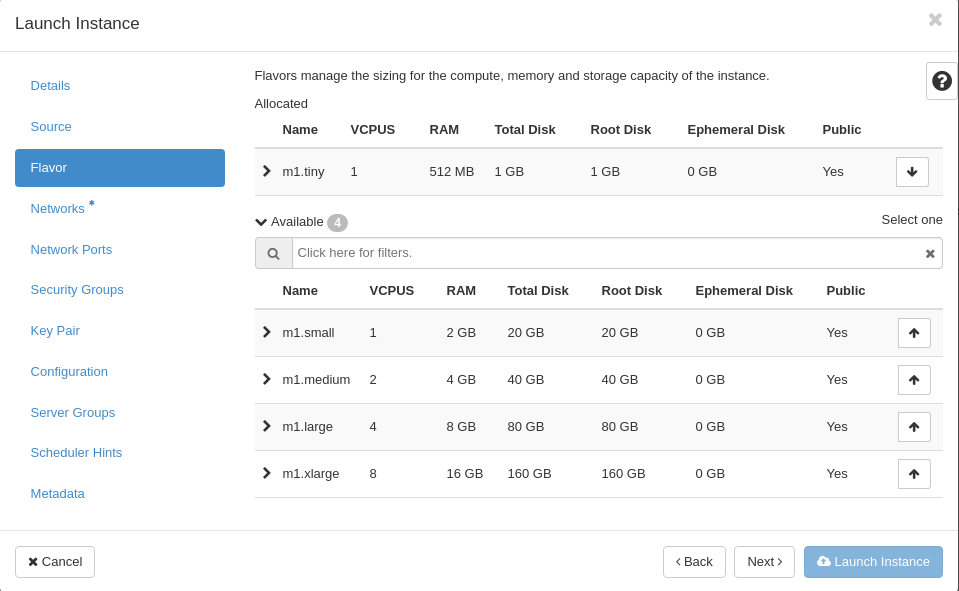
\includegraphics[width=.85\linewidth]{images/instanceflavor}
	\figcaption{Flavor für Instanz auswhählen}
\end{minipage}

Im letzten Schritt wird nun das bereits definierte Netzwerk ausgewählt:

\begin{minipage}{\linewidth}
	\centering
	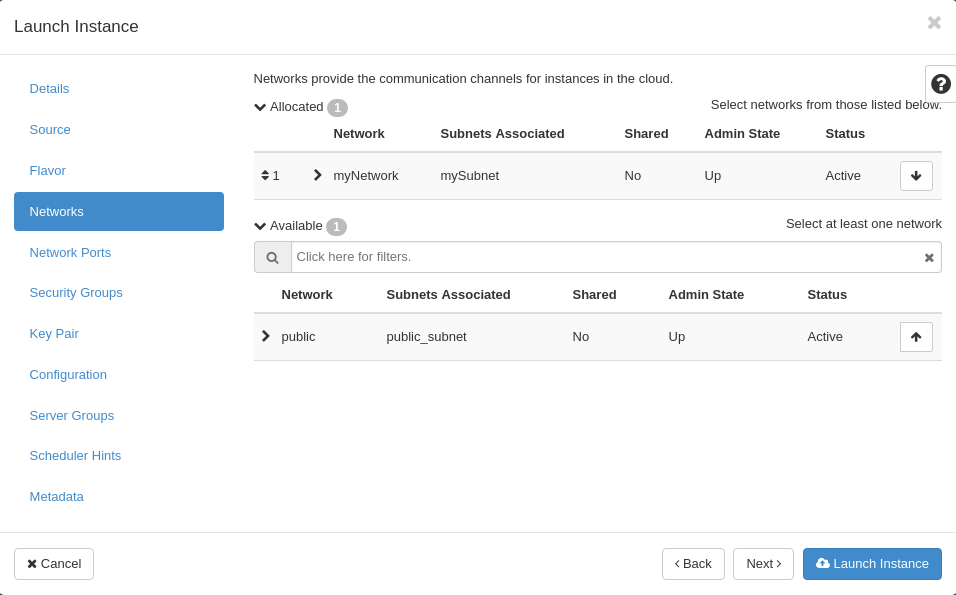
\includegraphics[width=.85\linewidth]{images/instancenetwork}
	\figcaption{Netzwerk für Instanz auswählen}
\end{minipage}

Nachdem die Instanz erstellt wurde, wird diese Initialisiert:

\begin{minipage}{\linewidth}
	\centering
	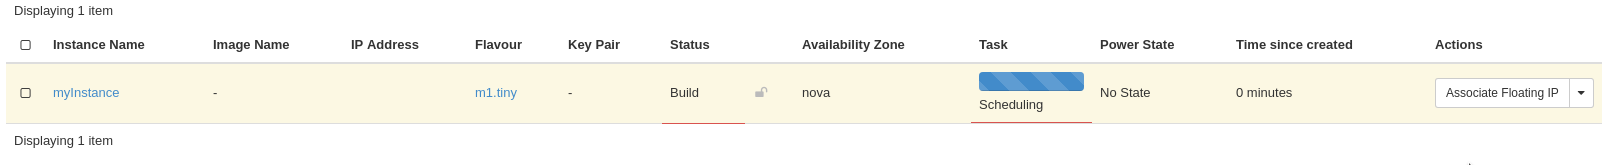
\includegraphics[width=1\linewidth]{images/instancestart}
	\figcaption{Instanz wird gestartet}
\end{minipage}

\subsection{Probleme}
Das Problem ist nun, nachdem die Instanz gestartet wurde, werden eine von den beiden Fehlern ausgegeben:

\begin{minipage}{\linewidth}
	\centering
	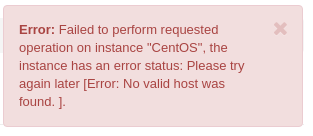
\includegraphics[width=0.6\linewidth]{images/error}
	\figcaption{Der Fehler hier dürfte sein, dass der Host nicht gefunden wird}
\end{minipage}

\begin{minipage}{\linewidth}
	\centering
	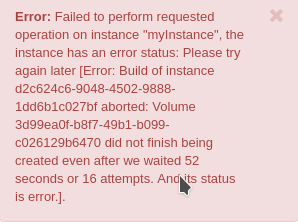
\includegraphics[width=0.6\linewidth]{images/error2}
	\figcaption{Der Fehler dürfte sein, dass das Erstellen zu viel Zeit braucht und somit abgebrochen wird}
\end{minipage}


